
%(BEGIN_QUESTION)
% Copyright 2013, Tony R. Kuphaldt, released under the Creative Commons Attribution License (v 1.0)
% This means you may do almost anything with this work of mine, so long as you give me proper credit

In this circuit, a generator turned by an automobile engine provides electrical power to various loads in the automobile as well as current to re-charge the automobile's battery.  The battery, of course, discharges when needed to provide additional current during ``heavy'' load conditions.  The wires connecting these components together have small amounts of resistance as shown:

$$\includegraphics[width=15.5cm]{i02408x01.eps}$$

Supposing the generator's terminal voltage is 14.1 VDC, the battery is {\it discharging} (i.e. acting as an electrical energy {\it source}) with a current of 25.3 amps, and the loads are drawing 45.9 amps of current, calculate the following:

\vskip 10pt

$V_{battery}$ = 

\vskip 10pt

$V_{loads}$ = 

\vskip 10pt

\underbar{file i02408}
%(END_QUESTION)





%(BEGIN_ANSWER)

$V_{battery}$ = 13.894 volts

\vskip 10pt

$V_{loads}$ = 12.517 volts

%(END_ANSWER)





%(BEGIN_NOTES)

{\bf This question is intended for exams only and not worksheets!}.

%(END_NOTES)


